% pLaTeX でタイプセットする
% platex masterabs && biber masterabs && platex masterabs && platex masterabs && dvipdfmx masterabs.dvi

%%%%%%%%%%%%%%%%%%%%%%%%%%%%%%%%%%%%%%%%%%%%%%%%%%%%%%%%%%%%%%%%
%%%%%%%  Example: extended abstract for master thesis
%%%%%%%  version 1.0
%%%%%%%  file name: template.tex
%%%%%%%%%%%%%%%%%%%%%%%%%%%%%%%%%%%%%%%%%%%%%%%%%%%%%%%%%%%%%%%%
%--------------- start preamble -------------------------------
\documentclass[a4paper]{jarticle} % 10pt fonts, default fonts
%\documentclass[a4paper,11pt]{jarticle} % 11pt fonts
%\documentclass[a4paper,12pt]{jarticle} % 12pt fonts
%--------------------------------------------------------------
\usepackage{masterabs} % 修士論文アブストラクトのスタイルファイル
%--------------------------------------------------------------
\usepackage{amsmath,amsthm,mathrsfs} % amslatex モードの指定
\usepackage{amsfonts,amssymb,txfonts} % amsfonts の指定
\usepackage[dvipdfmx]{graphicx} % 図の挿入の指定 (\includegraphicsなど)
%--------------------------------------------------------------
\columnseprule = 0.4pt % two columnの真ん中に縦線を引く
%--------   英文の場合: 表,図、参考文献を英語に変更 ----------------
\initenglish % 本文が英文の場合は % を取る(表=>Tab., 図=>Fig.など)
%--------------------------------------------------------------------
%

\theoremstyle{definition}
\newtheorem{thm}{Theorem}[section]
\newtheorem{dfn}[thm]{Definition}
\newtheorem{eg}[thm]{Example}
\newtheorem{lem}[thm]{Lemma}
\newtheorem{cor}[thm]{Corollary}
\theoremstyle{remark}
\newtheorem{rem}[thm]{Remark}

\DeclareMathOperator{\rank}{rank}
\DeclareMathOperator{\NS}{NS}
\DeclareMathOperator{\Tr}{Tr}
\DeclareMathOperator{\chara}{char}
\DeclareMathOperator{\Spec}{Spec}
\DeclareMathOperator{\ch}{ch}
\newcommand{\Neron}{N\'eron}

\usepackage[T1]{fontenc}

\usepackage[sorting=nyt,date=year,isbn=false,doi=false,url=false,giveninits]{biblatex} % biblatexを使用するためのパッケージ
\addbibresource{references.bib}

%-------------- end preamble ----------------------------------
%
%%%%%%    TEXT START    %%%%%%

\begin{document}
%
%-------------- two column -------------------------
\twocolumn[ % two column の場合は,先頭の % を取る
%---------------------------------------------------
%
%---------------------------------------------------------------------------
\no_tlfnmark % タイトルの最後にfootnote markを付けない場合は,先頭の % を取る
%---------------------------------------------------------------------------
%%% タイトルが 1行 \title{タイトル}を使う
%%% タイトルが 2 行にわたるときは \2ltitle{1行目}{2行目}を使う
%---------------------------------------------------------------
% \title{On the Mordell-Weil groups of elliptic surfaces associated with Frey curves of degree two} % 1 行用
%
\2ltitle{On the Mordell-Weil groups of elliptic surfaces}{associated with Frey curves of degree two} % 2 行用
%
%-------------------------------------------
% 日本語指導教員,著者名など
%-------------------------------------------
\begin{preliminary}
\profname{栗原将人教授}       %% 指導教員の名前 + 講師,准教授,教授
\name{82313206}{八木颯仁} %% 学籍番号, 著者名
\end{preliminary}
%
%---------- two column ----------------------
]% two columnの場合は,先頭の % を取る
%--------------------------------------------
%
%------- footnote に英文のタイトルを記述したいとき ----------------
% \etitle{On the Mordell-Weil groups of elliptic surfaces associated with Frey curves of degree two}
%----------------------------------------------------------------
%
\init_fnmark % 脚注マークの初期化(アラビア数字に変更)
%%%%%%%%%%%%%%%%%%%%%%%%%%%%  本文 %%%%%%%%%%%%%%%%%%%%%%%%%%%%%

\section{Introduction}
An elliptic curve defined over a field $K$ is a curve defined by a Weierstrass equation
\begin{equation*}
    E: y^{2} = x^{3} + Ax^2 + Bx + C
\end{equation*}
where $A,B,C \in K$ and the discriminant $\Delta = -4A^3C + A^2B^2 + 18ABC - 4B^3 - 27C^2$ is nonzero.
On points on an elliptic curve defined over $\mathbb{Q}$, we can define an addition law geometrically.
For two points $P,Q$ on $E$, the point $-(P+Q)$ is defined as the third point of intersection of the line passing through $P$ and $Q$ with the curve.
The sum $P+Q$ is the point symmetric to $-(P+Q)$ with respect to the $x$-axis.
\begin{figure}[ht]
    \centering
    \caption{$E: y^2 = x(x-3^2)(x+4^2)$}
    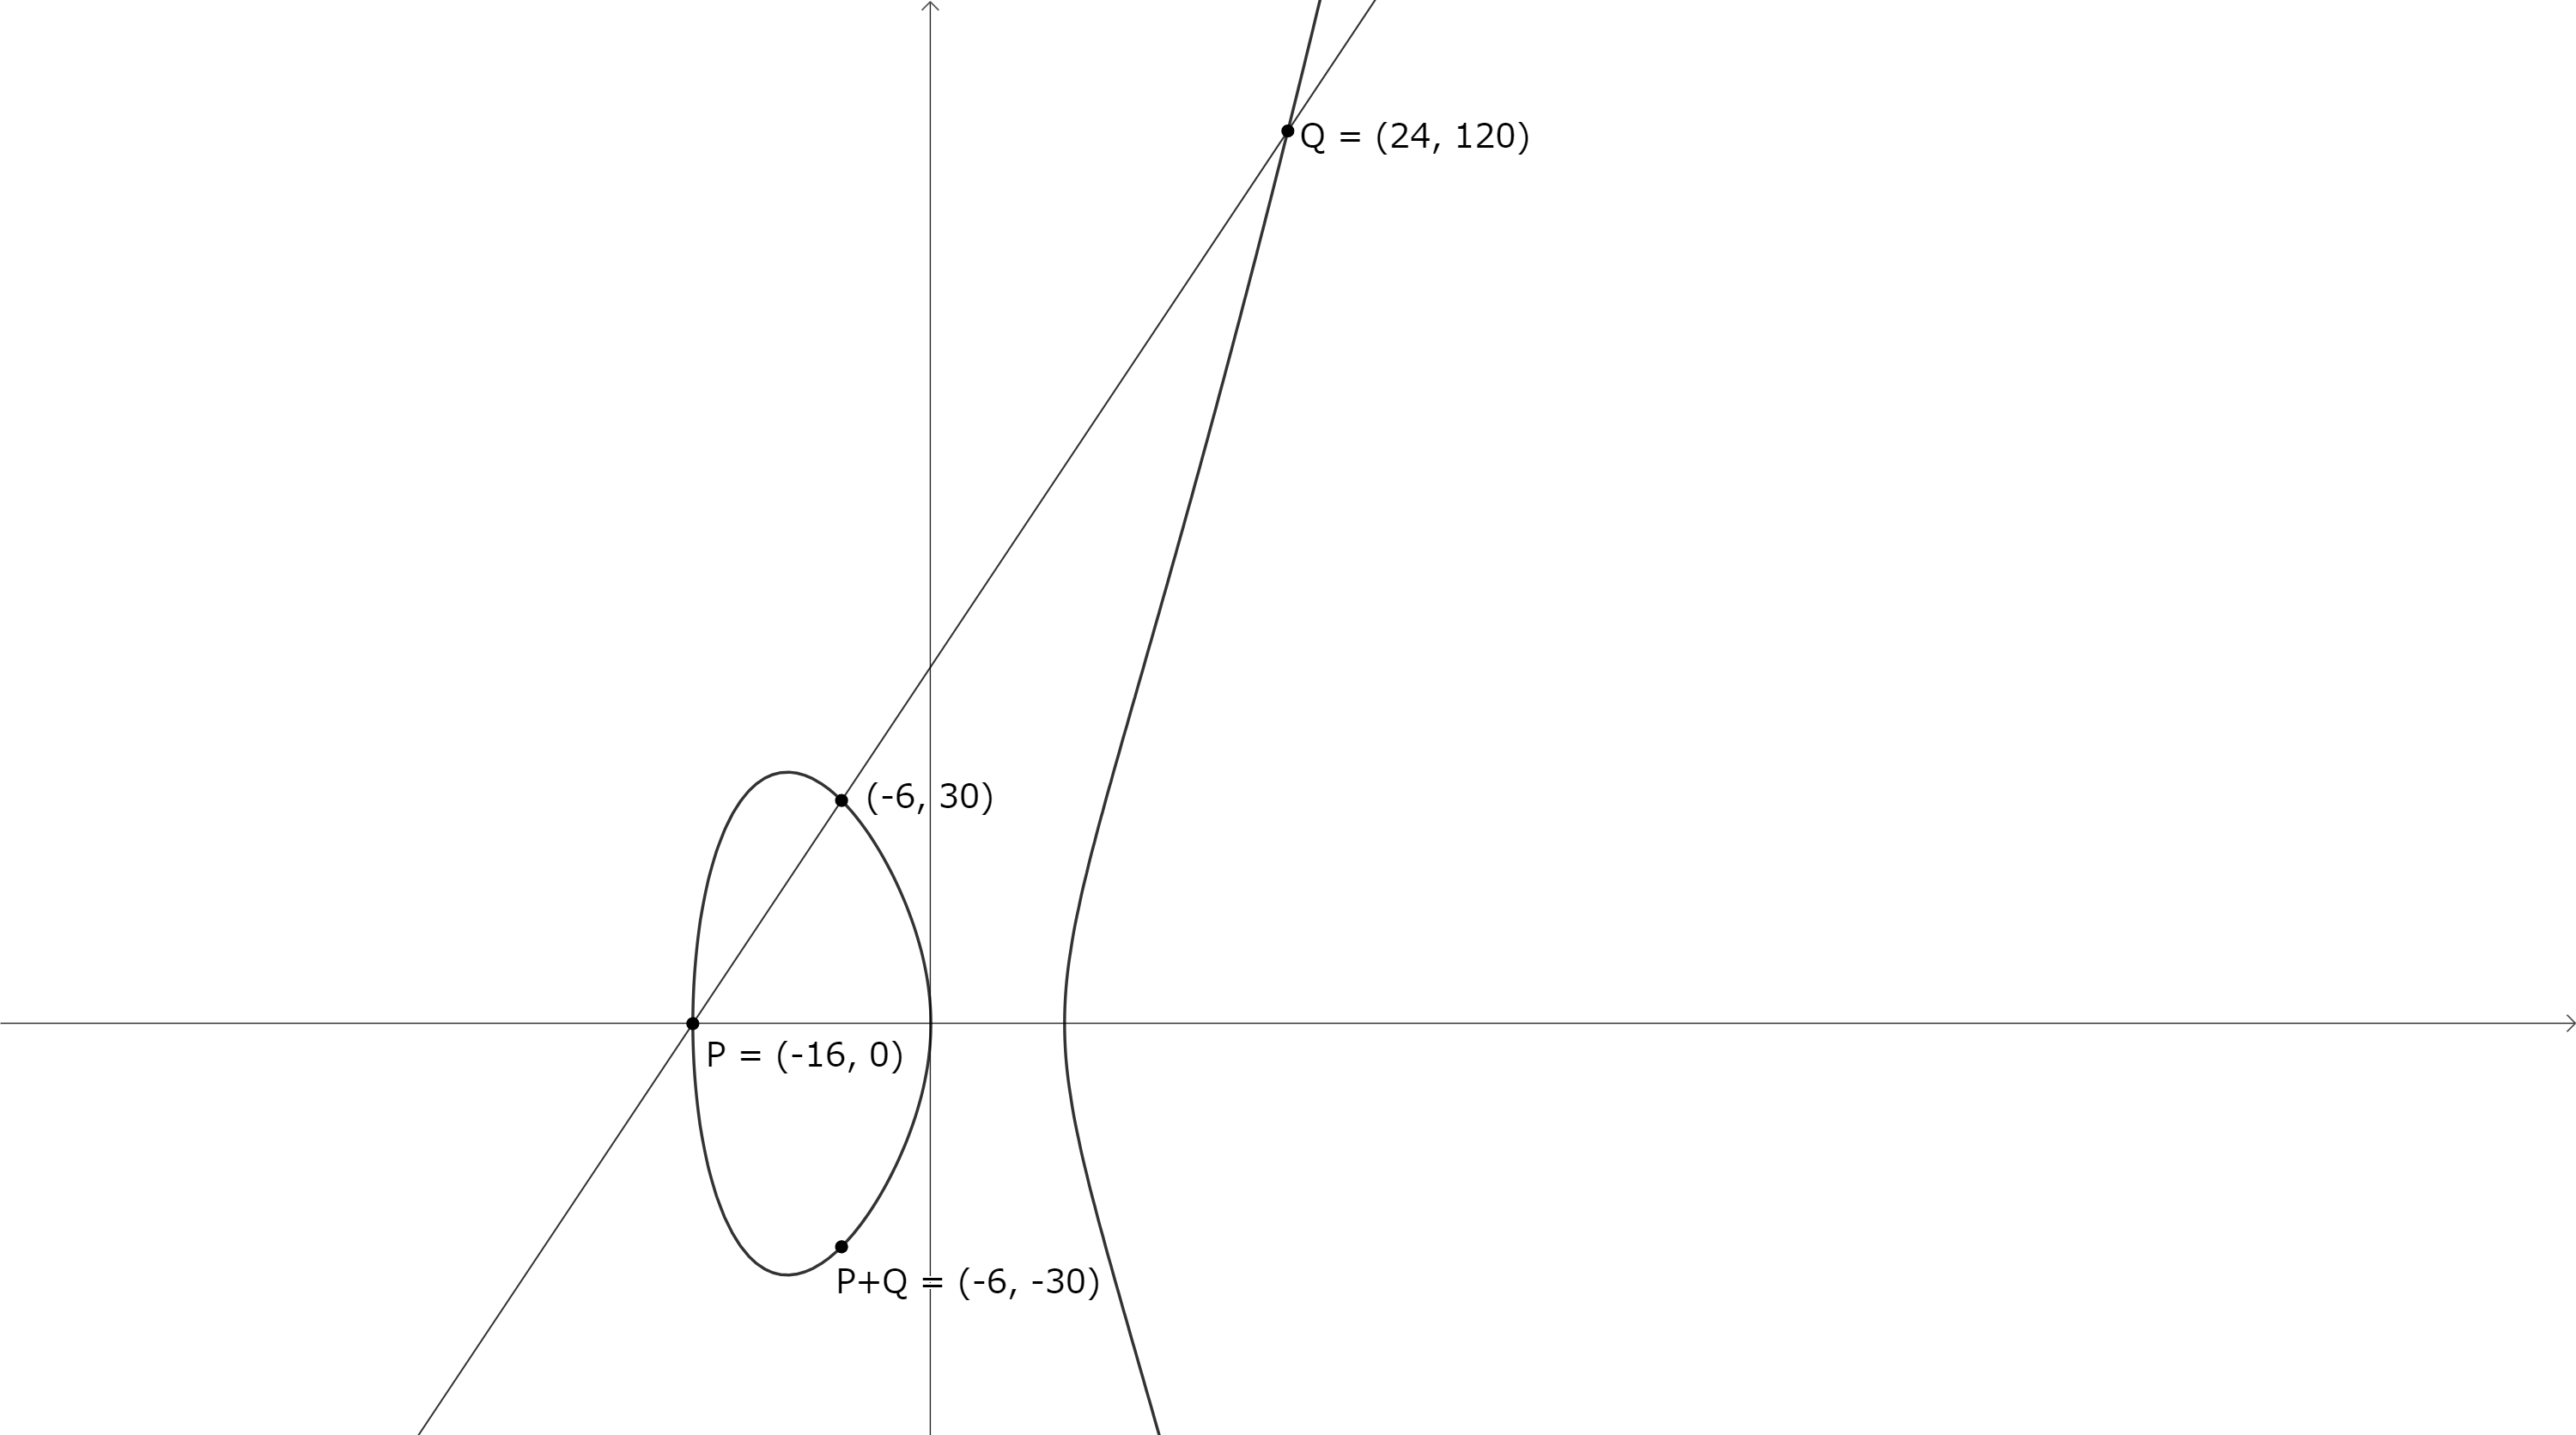
\includegraphics[keepaspectratio, width=\linewidth]{figures/3-4-5.png}
    \label{fig:elliptic_curve}
\end{figure}

The definition can be extended to any field $K$.
The set of points on an elliptic curve forms an abelian group with the identity element being the point at infinity.
The Mordell-Weil group $E(K)$ is a group consisting of all $K$-rational points on $E$.
The Mordell-Weil theorem states that the Mordell-Weil group is a finitely generated abelian group.
The Mordell-Weil group is an important object in the study of elliptic curves.
Especially, the rank of the Mordell-Weil group is important and difficult to determine.

In this paper, we consider elliptic curves in the form of the Frey curves for $n=2$.
In other words, let $(a,b,c) \in \mathbb{Z}^3$ be a Pythagorean triple and consider the elliptic curve defined by the Weierstrass equation
\begin{equation}
    \label{eq:2frey}
    y^{2} = x(x - a^{2})(x + b^{2}).
\end{equation}

We can parameterize Pythagorean triples $(a,b,c)$ by $m,n \in \mathbb{Z}$ with $(m,n)=1$ as $(a,b,c) = (2mn, m^{2} - n^{2}, m^{2} + n^{2})$.
Then the equation \eqref{eq:2frey} can be written as $y^{2} = x(x - 4m^2n^2)(x + (m^{2} - n^2)^{2})$.
We replace $x,y$ by $n^2x, n^3y$ and put $s = m/n$.
Then we get an elliptic curve
\begin{equation}
    \label{eq:E_{1,s}}
    E_{1,s}: y^{2} = x(x - 4s^{2})(x + (s^{2} - 1)^{2}).
\end{equation}
We consider $E_{1,s}$ as an elliptic curve over a function field $\overline{\mathbb{Q}}(s)$.
We associate an elliptic surface $\mathcal{E}_{1,s} \to \mathbb{P}^1$ to $E_{1,s}$.


\section{Main Theorem}

\begin{thm}
    \label{thm:E_{1,s}}
    The Mordell-Weil group of $E_{1,s}$ over $\overline{\mathbb{Q}}(s)$ satisfies
    \begin{equation*}
        E_{1,s}(\overline{\mathbb{Q}}(s)) \cong \mathbb{Z} / 4 \mathbb{Z} \oplus \mathbb{Z} / 4 \mathbb{Z},
    \end{equation*}
    especially the rank is $0$. The torsion subgroup is generated by
    \begin{align*}
        T_1 & := (2s(s+1)^2, 2s(s+1)^2(s^2+1)),                               \\
        T_2 & := (2 \sqrt{-1} s(s^2-1),2 \sqrt{-1} s(s+\sqrt{-1})^2(s^2-1)).
    \end{align*}
\end{thm}

By substituting $s = \frac{2t}{t^{2} - 3}$ into $E_{1,s}$, we get a new family of elliptic curves
\begin{equation*}
    E_{2,t}: y^{2} = x \left(x - 4 \left(\frac{2t}{t^{2} - 3} \right)^{2} \right) \left(x + \left(\left(\frac{2t}{t^{2} - 3} \right)^{2} - 1 \right)^{2} \right),
\end{equation*}
which is a subfamily of $E_{1,s}$.
The following is our main result.
\begin{thm}
    \label{thm:E_{2,t}}
    The Mordell-Weil group of $E_{2,t}$ over $\overline{\mathbb{Q}}(t)$ satisfies
    \begin{equation*}
        E_{2,t}(\overline{\mathbb{Q}}(t)) \cong \mathbb{Z} \oplus \mathbb{Z} / 4 \mathbb{Z} \oplus \mathbb{Z} / 4 \mathbb{Z},
    \end{equation*}
    especially the rank is $1$.
    The torsion subgroup is generated by $T_1$ and $T_2$ in Theorem~\ref{thm:E_{1,s}} with $s = \frac{2t}{t^{2} - 3}$.
\end{thm}
The important point is that we prove that the generic rank of $E_{2,t}$ is exactly $1$, not only the existence of a point of infinite order.
Our proof is based on the method of Naskręcki in \cite{ref:naskrecki2013}.


\section{Preliminaries}

In order to get the lower bound of the rank of the Mordell-Weil group, finding points of infinite order is enough.
It is quite difficult to get a good upper bound of the rank.
The following theorem behaves a key role in the proof of the main theorem.
\begin{thm}{(Shioda-Tate formula, \cite[Corollary 5.3]{ref:shioda1990})}
    \label{thm:shioda}
    Let $\mathcal{E} \to C$ be an elliptic surface over a smooth projective curve $C$ over an algebraically closed field $k$.
    Let $R \subset C$ be the set of points where the special fiber of $\mathcal{E}$ is singular.
    For each $v \in R$, let $m_{v}$ be the number of components of the special fiber of $\mathcal{E}$ at $v$.
    Let $\rho(\mathcal{E})$ denote the rank of the \Neron-Severi group of $\mathcal{E}$.
    Then, we have
    \begin{equation*}
        \rho (\mathcal{E}) = 2 + \sum_{v \in R} (m_{v} - 1) + \rank(E(k(C))).
    \end{equation*}
\end{thm}

\section{Reductions}
Let $A$ be a discrete valuation ring with maximal ideal $\mathfrak{m}$ and fraction field $K$.
Assume that the residue field $k=A/\mathfrak{m}$ has $q=p^r$ elements with $p$ prime.
Let $S$ be an integral scheme with a morphism $S \to \Spec A$ that is projective and smooth of relative dimension $2$.
Then the projective surface $\overline{S}=S_{\overline{\mathbb{Q}}}$ and $\tilde{S}=S_{\overline{k}}$ are smooth over the algebraically closed field $\overline{\mathbb{Q}}$ and $\overline{k}$, respectively.
We will assume that $\overline{S}$ and $\tilde{S}$ are integrals, i.e., they are irreducible, nonsingular, projective surfaces.

For a prime number $l \neq p$, we denote by $H_{\text{\'et}}^{2}(\tilde{S}, \mathbb{Q}_l)$ the $l$-adic \'etale cohomology group of $X$ and by $H_{\text{\'et}}^{2}(\tilde{S}, \mathbb{Q}_l)(1)$ its Tate twist.

Let $F: S_k \to S_k$ denote the absolute Frobenius, which acts as the identity on the points and by $f \mapsto f^p$ on the structure sheaf.
Set $\varphi:=F^{r}$ and let $\varphi^{(i)}$ denote the automorphism on $H_{\text{\'et}}^{i}(\tilde{S}, \mathbb{Q}_l)$ induced by $\varphi \times 1$ acting on $S_k \times_{\Spec k} \Spec \overline{k} \cong \tilde{S}$.

\begin{thm}{(\cite[Corollary 6.4.]{ref:vanluijk2007})}
    \label{cor:ns_upper_bound}
    The ranks of $\NS (\overline{S})$ and $\NS (\tilde{S})$ are bounded from above by the number of eigenvalues $\lambda$ of $\varphi^{(2)}$ for which $\lambda/q$ is a root of unity, counted with multiplicity.
\end{thm}

\begin{equation}
    \label{eq:rankdecomposition}
    \begin{aligned}
        \rank E_{2,t}(\overline{\mathbb{Q}}(t)) &= \rank E_{1,s}(\overline{\mathbb{Q}}(s)) \\
                                                &+ \rank E_{0,u}^{(1 + 3u)}(\overline{\mathbb{Q}}(u)) \\
                                                &+ \rank E_{0,u}^{(u(1 + 3u))}(\overline{\mathbb{Q}}(u)). \\
    \end{aligned}
\end{equation}

\begin{equation*}
    \chara(\varphi^{(2)}) = (x - 5)^{19}(x^{3} + x^{2} + 11 x - 77).
\end{equation*}
By Corollary~\ref{cor:ns_upper_bound}, $\rho(\mathcal{E}_{0,u}^{(1 + 3u)}) \leq 19$.
Then by Theorem~\ref{thm:shioda}, we have
\begin{equation*}
    \rank E_{0,u}^{(1 + 3u)}(\overline{\mathbb{Q}}(u)) \leq 19 - (2 + (2 - 1) + (4 - 1) \times 2 + (5 - 1) + (7 - 1)) = 0.
\end{equation*}

%%%%%%%%%%%%% 参考文献 %%%%%%%%%%%
\printbibliography

\end{document}